 % Project technical report — pdfLaTeX (Overleaf: set Main document to this file;
% upload transcript_ascii.txt in the SAME folder as this .tex — no tools/ path.)
\documentclass[11pt,a4paper]{article}

\usepackage[margin=1in]{geometry}
\usepackage[T1]{fontenc}
\usepackage{lmodern}
\usepackage{microtype}
\usepackage{booktabs}
\usepackage{enumitem}
\usepackage{amsmath}
\usepackage{xcolor}
\usepackage{listings}
\usepackage[most]{tcolorbox}% loads listings + breakable (for multi-page log box)
\usetikzlibrary{arrows.meta,positioning,calc,matrix,shapes.geometric,fit,backgrounds,quotes}
% hyperref must be loaded after listings/tcolorbox (avoids broken links / Overleaf warnings)
\usepackage{hyperref}

% Shared diagram styles (TikZ / pdfLaTeX, no external assets)
\tikzset{
  diagarr/.style={-{Latex[length=1.8mm]}, thick, draw=gray!65},
  diagnode/.style={draw, rounded corners=2pt, align=center, inner sep=4pt},
  diagsmall/.style={font=\scriptsize},
}

\lstset{
  basicstyle=\ttfamily\scriptsize,
  breaklines=true,
  breakatwhitespace=true,
  columns=fullflexible,
  frame=single,
  xleftmargin=0.5em,
}
\lstdefinestyle{runlog}{
  basicstyle=\ttfamily\footnotesize,
  breaklines=true,
  breakatwhitespace=true,
  columns=fullflexible,
  frame=none,
  xleftmargin=0pt,
  xrightmargin=0pt,
  framexleftmargin=0pt,
  framexrightmargin=0pt,
  aboveskip=0.25em,
  belowskip=0.25em,
  tabsize=2,
  showstringspaces=false,
}

\hypersetup{
  colorlinks=true,
  linkcolor={blue!60!black},
  urlcolor={blue!70!black},
  citecolor={blue!60!black},
}

\title{\textbf{Autonomous Research Outreach Agent}\\[0.35em]
\large Technical Report: Workflow, Logic, and Architecture}
\author{ML Project --- Autonomous Agent}
\date{\today}

\begin{document}
\maketitle

\begin{abstract}
This report describes an end-to-end system for academic outreach: from a vague user goal through structured intent capture, execution planning, web discovery of faculty, relevance ranking, and personalized email drafting, with human supervision before sending and optional scheduled automation for replies and follow-ups. The implementation combines conversational LLM agents, a LangGraph-style orchestration graph, web search and scraping, composite relevance scoring, and a small persistence layer (SQLite) with Gmail integration.
\end{abstract}

\tableofcontents
\newpage

% ---------------------------------------------------------------------------
\section{Introduction and objectives}

The project implements an \emph{agentic} pipeline that helps a student or researcher run a disciplined cold-email campaign toward faculty. The design emphasizes:
\begin{itemize}[noitemsep]
  \item \textbf{Structured intent} --- slot-filling so vague goals become actionable constraints (domains, geography, timeline, profile).
  \item \textbf{Explicit plans} --- a machine-readable execution plan (search, filters, email style, schedule) that the user can approve or refine.
  \item \textbf{Grounded outreach} --- candidates are discovered from the open web and bibliographic APIs; emails reference real publications and lab context where possible.
  \item \textbf{Human oversight} --- the first pass is supervised: the user confirms intent and plan, then reviews drafts before messages leave the system.
  \item \textbf{Gradual autonomy} --- after approval and configuration, scheduled jobs can re-crawl for new leads, detect inbox replies, and send bounded follow-ups.
\end{itemize}

% ---------------------------------------------------------------------------
\section{High-level architecture}

Figure~\ref{fig:layers} summarizes how packages connect around shared \texttt{AgentState}; Figure~\ref{fig:repo-tree} lists top-level folders in a non-overlapping grid. Figures~\ref{fig:cli-five}--\ref{fig:supervised-flow} map the Typer CLI to control and data movement. Figure~\ref{fig:arch-flow} groups the longer 14-step narrative into phases.

\begin{figure}[htbp]
\centering
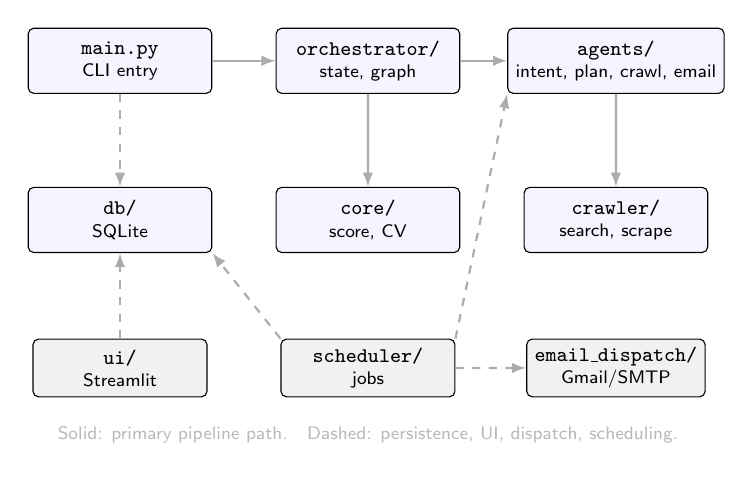
\begin{tikzpicture}[
  scale=0.94, transform shape,
  font=\footnotesize\sffamily,
  module/.style={diagnode, fill=blue!4, minimum width=2.48cm, minimum height=0.88cm, inner sep=3pt},
  infra/.style={diagnode, fill=gray!11, minimum width=2.35cm, minimum height=0.78cm, inner sep=3pt},
  note/.style={font=\scriptsize\sffamily, text=gray!55, align=center},
]
  \node[module] (main)   at (0,0)     {\textbf{\texttt{main.py}}\\[-1pt]{\scriptsize CLI entry}};
  \node[module] (orch)   at (3.35,0)  {\textbf{\texttt{orchestrator/}}\\[-1pt]{\scriptsize state, graph}};
  \node[module] (agents) at (6.7,0)   {\textbf{\texttt{agents/}}\\[-1pt]{\scriptsize intent, plan, crawl, email}};

  \node[module] (db)     at (0,-2.15) {\textbf{\texttt{db/}}\\[-1pt]{\scriptsize SQLite}};
  \node[module] (core)   at (3.35,-2.15){\textbf{\texttt{core/}}\\[-1pt]{\scriptsize score, CV}};
  \node[module] (crawl)  at (6.7,-2.15){\textbf{\texttt{crawler/}}\\[-1pt]{\scriptsize search, scrape}};

  \node[infra] (ui)      at (0,-4.15) {\textbf{\texttt{ui/}}\\[-1pt]{\scriptsize Streamlit}};
  \node[infra] (sched)   at (3.35,-4.15){\textbf{\texttt{scheduler/}}\\[-1pt]{\scriptsize jobs}};
  \node[infra] (email)   at (6.7,-4.15){\textbf{\texttt{email\_dispatch/}}\\[-1pt]{\scriptsize Gmail/SMTP}};

  \draw[diagarr] (main) -- (orch);
  \draw[diagarr] (orch) -- (agents);
  \draw[diagarr] (orch) -- (core);
  \draw[diagarr] (agents) -- (crawl);

  \draw[diagarr, dashed] (main) -- (db);
  \draw[diagarr, dashed] (ui) -- (db);
  \draw[diagarr, dashed] (sched.north west) -- (db.south east);
  \draw[diagarr, dashed] (sched) -- (email);
  \draw[diagarr, dashed] (sched.north east) -- (agents.south west);

  \node[note] at (3.35,-5.05) {Solid: primary pipeline path.\quad Dashed: persistence, UI, dispatch, scheduling.};
\end{tikzpicture}
\caption{Repository modules and their main dependencies. \texttt{AgentState} lives in \texttt{orchestrator/}; the CLI path exercises agents, crawler, core scoring, and the database before optional dispatch and scheduled jobs.}
\label{fig:layers}
\end{figure}

\begin{figure}[htbp]
\centering
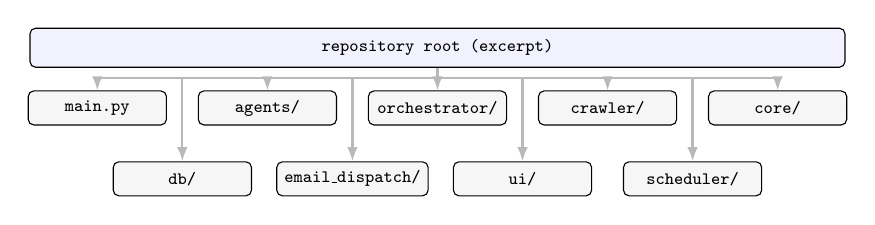
\begin{tikzpicture}[
  scale=0.9, transform shape,
  font=\scriptsize\ttfamily,
  pkg/.style={diagnode, fill=gray!7, inner sep=3pt, minimum width=1.95cm, minimum height=0.48cm},
]
  \node[pkg, fill=blue!5, minimum width=11.5cm, minimum height=0.55cm] (cap) at (4.8,0.85) {\textbf{repository root (excerpt)}};
  
  \node[pkg] (pk1) at (0,0) {\textbf{main.py}};
  \node[pkg] (pk2) at (2.4,0) {\textbf{agents/}};
  \node[pkg] (pk3) at (4.8,0) {\textbf{orchestrator/}};
  \node[pkg] (pk4) at (7.2,0) {\textbf{crawler/}};
  \node[pkg] (pk5) at (9.6,0) {\textbf{core/}};
  
  \node[pkg] (pk6) at (1.2,-1.0) {\textbf{db/}};
  \node[pkg] (pk7) at (3.6,-1.0) {\textbf{email\_dispatch/}};
  \node[pkg] (pk8) at (6.0,-1.0) {\textbf{ui/}};
  \node[pkg] (pk9) at (8.4,-1.0) {\textbf{scheduler/}};
  
  \foreach \n in {pk1,pk2,pk3,pk4,pk5,pk6,pk7,pk8,pk9}
    \draw[diagarr, gray!55] (cap.south) -- ++(0,-0.15) -| (\n.north);
\end{tikzpicture}
\caption{Top-level packages and entry script ordered to mathematically prevent intersecting lines.}
\label{fig:repo-tree}
\end{figure}


\begin{figure}[htbp]
\centering
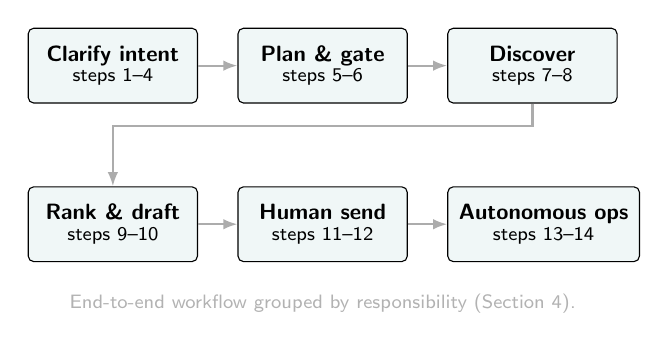
\begin{tikzpicture}[
  font=\footnotesize\sffamily,
  node distance=0.42cm and 0.5cm,
  ph/.style={diagnode, fill=teal!6, minimum width=2.15cm, minimum height=0.95cm},
]
  \node[ph] (p1) {\textbf{Clarify intent}\\[-2pt]{\scriptsize steps 1--4}};
  \node[ph, right=of p1] (p2) {\textbf{Plan \& gate}\\[-2pt]{\scriptsize steps 5--6}};
  \node[ph, right=of p2] (p3) {\textbf{Discover}\\[-2pt]{\scriptsize steps 7--8}};
  \node[ph, below=1.05cm of p1] (p4) {\textbf{Rank \& draft}\\[-2pt]{\scriptsize steps 9--10}};
  \node[ph, right=of p4] (p5) {\textbf{Human send}\\[-2pt]{\scriptsize steps 11--12}};
  \node[ph, right=of p5] (p6) {\textbf{Autonomous ops}\\[-2pt]{\scriptsize steps 13--14}};
  \foreach \a/\b in {p1/p2,p2/p3,p4/p5,p5/p6}
    \draw[diagarr] (\a) -- (\b);
  \draw[diagarr] (p3.south) -- ++(0,-0.28) -| (p4.north);
  \node[font=\scriptsize\sffamily, text=gray!60, below=0.28cm of p5.south]{End-to-end workflow grouped by responsibility (Section~4).};
\end{tikzpicture}
\caption{Phased view of the 14-step workflow: from slot-filling through discovery, scoring, supervised sending, and optional scheduled re-crawl, replies, and follow-ups.}
\label{fig:arch-flow}
\end{figure}

\begin{figure}[htbp]
\centering
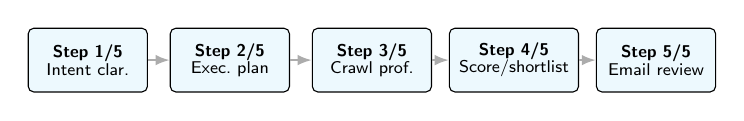
\begin{tikzpicture}[
  scale=0.88, transform shape,
  font=\scriptsize\sffamily,
  st/.style={diagnode, fill=cyan!7, minimum width=1.72cm, minimum height=0.92cm, align=center},
]
  \node[st] (s1) at (0,0) {\textbf{Step 1/5}\\[-1pt]Intent clar.};
  \node[st] (s2) at (2.05,0) {\textbf{Step 2/5}\\[-1pt]Exec.\ plan};
  \node[st] (s3) at (4.1,0) {\textbf{Step 3/5}\\[-1pt]Crawl prof.};
  \node[st] (s4) at (6.15,0) {\textbf{Step 4/5}\\[-1pt]Score/shortlist};
  \node[st] (s5) at (8.2,0) {\textbf{Step 5/5}\\[-1pt]Email review};
  \foreach \a/\b in {s1/s2,s2/s3,s3/s4,s4/s5}
    \draw[diagarr] (\a) -- (\b);
\end{tikzpicture}
\caption{Supervised \texttt{main.py start} pipeline as labeled in the CLI (matches \texttt{main.py}).}
\label{fig:cli-five}
\end{figure}

\begin{figure}[htbp]
\centering
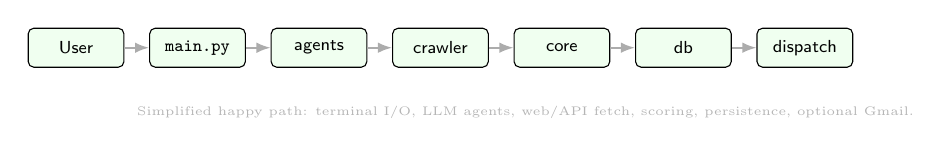
\begin{tikzpicture}[
  scale=0.9, transform shape,
  font=\scriptsize\sffamily,
  ax/.style={diagnode, fill=green!6, minimum width=1.35cm, minimum height=0.55cm},
]
  \node[ax] (U) at (0,0) {User};
  \node[ax, right=0.35cm of U] (C) {\texttt{main.py}};
  \node[ax, right=0.35cm of C] (A) {agents};
  \node[ax, right=0.35cm of A] (W) {crawler};
  \node[ax, right=0.35cm of W] (K) {core};
  \node[ax, right=0.35cm of K] (D) {db};
  \node[ax, right=0.35cm of D] (M) {dispatch};
  \foreach \a/\b in {U/C,C/A,A/W,W/K,K/D,D/M}
    \draw[diagarr] (\a) -- (\b);
  \node[font=\tiny, text=gray!58, below=0.42cm of W.south, xshift=1.2cm]
    {Simplified happy path: terminal I/O, LLM agents, web/API fetch, scoring, persistence, optional Gmail.};
\end{tikzpicture}
\caption{Simplified supervised-run data path (one direction of influence; loops for HITL omitted).}
\label{fig:supervised-flow}
\end{figure}

\noindent
\textbf{Two orchestration paths.} The primary user flow in \texttt{main.py} runs a \emph{sequential} supervised pipeline (five labeled CLI steps). An alternative \texttt{orchestrator/graph.py} compiles a \textbf{LangGraph} \texttt{StateGraph} with nodes \texttt{intent} $\rightarrow$ \texttt{planning} $\rightarrow$ \texttt{crawling} $\rightarrow$ \texttt{scoring} $\rightarrow$ \texttt{email\_draft} $\rightarrow$ \texttt{send} (emulated), using a memory checkpointer for stateful runs. Both paths share the same Pydantic/TypedDict state models (Figure~\ref{fig:dual-orchestrate}).

\begin{figure}[htbp]
\centering
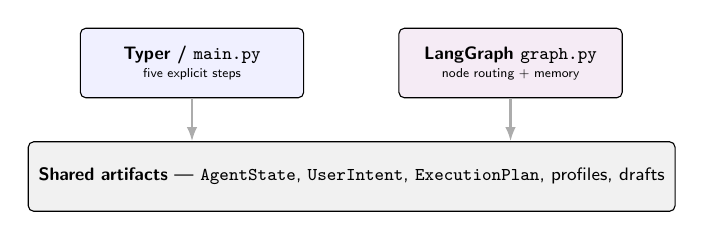
\begin{tikzpicture}[
  scale=0.93, transform shape,
  font=\scriptsize\sffamily,
  br/.style={diagnode, minimum width=3.05cm, minimum height=0.95cm, align=center},
]
  \node[br, fill=blue!6] (cli) at (0,0) {\textbf{Typer / \texttt{main.py}}\\[-1pt]{\tiny five explicit steps}};
  \node[br, fill=violet!8] (lg) at (4.35,0) {\textbf{LangGraph \texttt{graph.py}}\\[-1pt]{\tiny node routing + memory}};
  \node[br, fill=gray!11, minimum width=6.2cm] (com) at (2.18,-1.55) {\textbf{Shared artifacts} --- \texttt{AgentState}, \texttt{UserIntent}, \texttt{ExecutionPlan}, profiles, drafts};
  \draw[diagarr] (cli.south) -- (cli.south |- com.north);
  \draw[diagarr] (lg.south) -- (lg.south |- com.north);
\end{tikzpicture}
\caption{Dual orchestration entry points converging on the same typed state and persistence contracts.}
\label{fig:dual-orchestrate}
\end{figure}

% ---------------------------------------------------------------------------
\section{Central state and data models}

All agents read and write a shared \texttt{AgentState} (\texttt{orchestrator/state.py}), a \texttt{TypedDict} holding the keys below; Figure~\ref{fig:agentstate} shows them schematically.
\begin{itemize}[noitemsep]
  \item \texttt{messages} --- chat history for clarification and plan explanation.
  \item \texttt{intent} --- serialized \texttt{UserIntent}.
  \item \texttt{plan} --- serialized \texttt{ExecutionPlan}.
  \item \texttt{professors}, \texttt{shortlisted} --- lists of \texttt{ProfessorProfile} dictionaries.
  \item \texttt{draft\_emails} --- \texttt{DraftEmail} records.
  \item \texttt{human\_input}, \texttt{mode}, \texttt{session\_id}, optional \texttt{error}.
\end{itemize}

\begin{figure}[htbp]
\centering
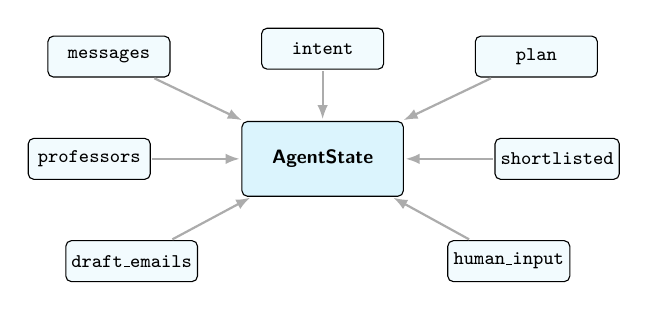
\begin{tikzpicture}[
  font=\scriptsize\ttfamily,
  blob/.style={diagnode, fill=cyan!5, minimum width=1.55cm, minimum height=0.52cm, inner sep=2pt},
  hub/.style={diagnode, fill=cyan!14, minimum width=2.05cm, minimum height=0.95cm, inner sep=3pt, font=\scriptsize\bfseries\sffamily},
]
  \node[hub] (A) {AgentState};
  \node[blob, above left=0.55cm and 0.9cm of A] (m) {messages};
  \node[blob, above=0.65cm of A] (i) {intent};
  \node[blob, above right=0.55cm and 0.9cm of A] (p) {plan};
  \node[blob, left=1.15cm of A] (pr) {professors};
  \node[blob, right=1.15cm of A] (sh) {shortlisted};
  \node[blob, below left=0.55cm and 0.55cm of A] (dr) {draft\_emails};
  \node[blob, below right=0.55cm and 0.55cm of A] (hi) {human\_input};
  \foreach \x in {m,i,p,pr,sh,dr,hi}
    \draw[diagarr, shorten >=0.6pt, shorten <=0.6pt] (\x) -- (A);
\end{tikzpicture}
\caption{Shared \texttt{AgentState} hub and the main fields agents read or update (Section~3).}
\label{fig:agentstate}
\end{figure}

\subsection{User intent (\texttt{UserIntent})}
Progressively filled slots include outreach \texttt{goal} (enum, e.g.\ research internship), \texttt{research\_domains}, \texttt{countries}, optional \texttt{target\_institutions}, \texttt{timeline}, \texttt{user\_name}, profile summary or \texttt{cv\_path}, email tone, follow-up and volume preferences, and structured CV-derived fields (degree, institution, highlights, projects, etc.). Method \texttt{missing\_required\_slots()} drives which questions the intent agent asks next; \texttt{confirmed} gates transition to planning in graph routing. Figure~\ref{fig:intent-slots} summarizes the loop.

\begin{figure}[htbp]
\centering
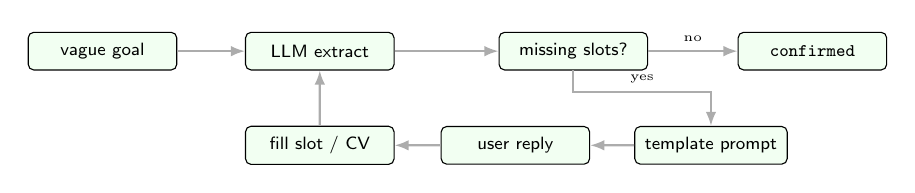
\begin{tikzpicture}[
  scale=0.92, transform shape,
  font=\scriptsize\sffamily,
  st/.style={diagnode, fill=green!5, minimum width=2.05cm, minimum height=0.52cm},
]
  % Top row
  \node[st] (a) at (0,0) {vague goal};
  \node[st] (b) at (3.0,0) {LLM extract};
  \node[st] (c) at (6.5,0) {missing slots?};
  \node[st] (g) at (9.8,0) {\texttt{confirmed}};

  % Bottom row
  \node[st] (f) at (3.0,-1.3) {fill slot / CV};
  \node[st] (e) at (5.7,-1.3) {user reply};
  \node[st] (d) at (8.4,-1.3) {template prompt};

  \draw[diagarr] (a) -- (b);
  \draw[diagarr] (b) -- (c);
  \draw[diagarr] (c) -- node[above, font=\tiny] {no} (g);

  \draw[diagarr] (c.south) -- ++(0,-0.3) -| node[pos=0.25, above, font=\tiny] {yes} (d.north);
  \draw[diagarr] (d) -- (e);
  \draw[diagarr] (e) -- (f);
  \draw[diagarr] (f) -- (b);

\end{tikzpicture}
\caption{Slot-filling loop for \texttt{UserIntent}: questions repeat until required fields exist, then confirmation releases planning.}
\label{fig:intent-slots}
\end{figure}

\subsection{Execution plan (\texttt{ExecutionPlan})}
Encodes \texttt{SearchStrategy} (keywords, country and institution filters), \texttt{FilteringCriteria} (minimum relevance score, require email, recency flags), \texttt{EmailStrategy} (personalization level, tone, word count, CV attachment), \texttt{SendingSchedule} (emails per week, follow-up delay, max follow-ups), and \texttt{top\_k\_professors}. The planning LLM is instructed to preserve geographic strings exactly (e.g.\ ``Punjab, India'') when copying filters.

\subsection{Professor and email artifacts}
\texttt{ProfessorProfile} stores identity, institution, keywords, publications, URLs, optional \texttt{accepting\_students}, crawl metadata, and \texttt{relevance\_score}. \texttt{DraftEmail} stores recipient, subject, body, status lifecycle (draft, approved, sent, replied, followed up), and timestamps. Figure~\ref{fig:email-lifecycle} sketches the draft lifecycle relative to automation.

\begin{figure}[htbp]
\centering
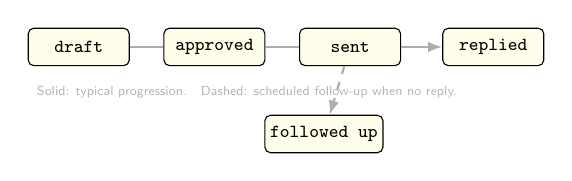
\begin{tikzpicture}[
  scale=0.95, transform shape,
  font=\scriptsize\ttfamily,
  st/.style={diagnode, fill=yellow!8, minimum width=1.35cm, minimum height=0.5cm, inner sep=2pt},
]
  \node[st] (d) at (0,0) {draft};
  \node[st, right=0.45cm of d] (a) {approved};
  \node[st, right=0.45cm of a] (s) {sent};
  \node[st, right=0.55cm of s] (r) {replied};
  \node[st, below=0.65cm of s, xshift=-0.35cm] (f) {followed up};
  \draw[diagarr] (d) -- (a) -- (s) -- (r);
  \draw[diagarr, dashed] (s) -- (f);
  \node[font=\tiny\sffamily, text=gray!58, below=0.15cm of d.south west, anchor=north west]
    {Solid: typical progression.\quad Dashed: scheduled follow-up when no reply.};
\end{tikzpicture}
\caption{\texttt{DraftEmail} status progression (conceptual; exact flags depend on DB rows and scheduler).}
\label{fig:email-lifecycle}
\end{figure}

% ---------------------------------------------------------------------------
\section{End-to-end workflow (14 steps)}

The following maps your specified workflow to the implementation. Steps~1--6 are predominantly handled by \texttt{IntentAgent} and \texttt{PlanningAgent}; steps~7--10 by \texttt{CrawlerAgent}, \texttt{RelevanceScorer}, and \texttt{EmailAgent}; steps~11--12 by CLI review, the database, and Streamlit/Gmail dispatch; steps~13--14 by \texttt{scheduler/}. Figure~\ref{fig:crawl-pipeline} compresses the discovery stack; Figure~\ref{fig:scheduler-jobs} shows scheduled maintenance tasks.

\begin{figure}[htbp]
\centering
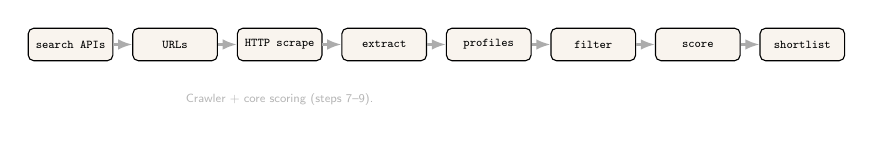
\begin{tikzpicture}[
  scale=0.86, transform shape,
  font=\tiny\ttfamily,
  bx/.style={diagnode, fill=brown!9, minimum width=1.25cm, minimum height=0.48cm, inner sep=1.5pt},
]
  \node[bx] (q) at (0,0) {search APIs};
  \node[bx, right=0.28cm of q] (u) {URLs};
  \node[bx, right=0.28cm of u] (h) {HTTP scrape};
  \node[bx, right=0.28cm of h] (x) {extract};
  \node[bx, right=0.28cm of x] (p) {profiles};
  \node[bx, right=0.28cm of p] (f) {filter};
  \node[bx, right=0.28cm of f] (z) {score};
  \node[bx, right=0.28cm of z] (l) {shortlist};
  \foreach \a/\b in {q/u,u/h,h/x,x/p,p/f,f/z,z/l}
    \draw[diagarr] (\a) -- (\b);
  \node[font=\tiny\sffamily, text=gray!58, below=0.35cm of h.south]{Crawler + core scoring (steps~7--9).};
\end{tikzpicture}
\caption{Discovery pipeline: queries and heuristics yield URLs; scraping and \texttt{ProfileExtractor} build \texttt{ProfessorProfile} rows, then filters and \texttt{RelevanceScorer} produce \texttt{shortlisted}.}
\label{fig:crawl-pipeline}
\end{figure}

\begin{enumerate}[leftmargin=*]
  \item \textbf{User provides a vague high-level goal.} \\
  CLI prompt \texttt{What do you want to do?} or first \texttt{human\_input} in the graph.

  \item \textbf{Agent extracts intent and identifies missing parameters.} \\
  \texttt{IntentAgent.extract\_initial\_intent} uses an LLM with a JSON schema prompt to populate \texttt{UserIntent}; \texttt{missing\_required\_slots()} lists gaps (domains, countries, timeline, name, profile/CV).

  \item \textbf{Agent asks structured follow-up questions.} \\
  Template map \texttt{SLOT\_QUESTIONS} in \texttt{intent\_agent.py}; \texttt{fill\_slot\_from\_reply} parses answers (including PDF CV via \texttt{CVParser}).

  \item \textbf{Agent builds structured state representation.} \\
  The running \texttt{UserIntent} model is serialized into \texttt{AgentState["intent"]}; optional persistence to \texttt{session\_state.json} and \texttt{upsert\_session\_state} in the DB.

  \item \textbf{Agent generates and displays execution plan.} \\
  \texttt{PlanningAgent.generate\_plan} produces \texttt{ExecutionPlan} JSON via LLM, with fallback \texttt{\_default\_plan}; \texttt{display\_plan} and a plain-language \texttt{PLAN\_EXPLANATION\_PROMPT} explain it to the user.

  \item \textbf{User approves plan.} \\
  In \texttt{run\_cli}, responses \texttt{yes}/\texttt{no} trigger confirm or \texttt{refine\_plan}. In LangGraph, \texttt{evaluate\_plan} routes to \texttt{crawling} only when \texttt{plan.confirmed} is true.

  \item \textbf{Agent crawls web sources.} \\
  \texttt{CrawlerAgent.run}: web search (\texttt{search\_professors}), URL heuristics (\texttt{is\_likely\_faculty\_url}), Semantic Scholar batch queries, optional snowball expansion, then \texttt{scrape\_batch} and \texttt{ProfileExtractor.batch\_extract}.

  \item \textbf{Agent extracts candidate professor data.} \\
  Structured \texttt{ProfessorProfile} instances with email, keywords, publications, etc.; optional filter requiring a discoverable email address.

  \item \textbf{Agent ranks candidates by relevance.} \\
  \texttt{RelevanceScorer.shortlist}: geographic pre-filter when countries are specific; composite score
  \begin{equation*}
    s = \sum_i w_i s_i, \quad
    w = (0.30, 0.20, 0.15, 0.25, 0.10)
  \end{equation*}
  for keyword overlap, LLM ``embedding'' slot (student--lab fit score), publication recency, geographic match, and student-acceptance signal; then threshold by \texttt{min\_relevance\_score} and take top-$K$.
  Figure~\ref{fig:score-weights} shows the relative weights.

  \item \textbf{Agent drafts personalized emails.} \\
  \texttt{EmailAgent.generate\_email}: salutation sanitization, student context from \texttt{build\_email\_internship\_context}, JSON generation prompt with length targets, QC/retry, optional critique pass, and template \texttt{\_fallback\_email} if quality checks fail.

  \item \textbf{User supervises first execution.} \\
  \texttt{main.py} loops per draft: \texttt{display\_email}, user chooses \texttt{approve}/\texttt{skip}; approved rows go to \texttt{db.save\_draft\_email}. Streamlit \texttt{python main.py review} supports further review and sending.

  \item \textbf{Emails are sent.} \\
  Gmail/SMTP clients under \texttt{email\_dispatch/}; sending updates persisted in the database (implementation details depend on UI and OAuth setup).

  \item \textbf{Agent tracks replies and sends follow-ups.} \\
  \texttt{ReplyMonitor.scan\_and\_update\_replies} matches inbox senders to sent rows and marks \texttt{replied}. \texttt{FollowupEngine.process\_pending\_followups} sends polite follow-ups after \texttt{followup\_days} without a reply, respecting max follow-up policy encoded in intent/plan.

  \item \textbf{After approval, system transitions to autonomous mode.} \\
  \texttt{AutonomousScheduler} (APScheduler) schedules \texttt{re\_crawl\_job} (discover new professors, skip already-contacted emails), \texttt{check\_replies\_job}, and \texttt{send\_followups\_job}. This phase assumes Gmail and DB configuration and user consent to automated actions.
\end{enumerate}

\begin{figure}[htbp]
\centering
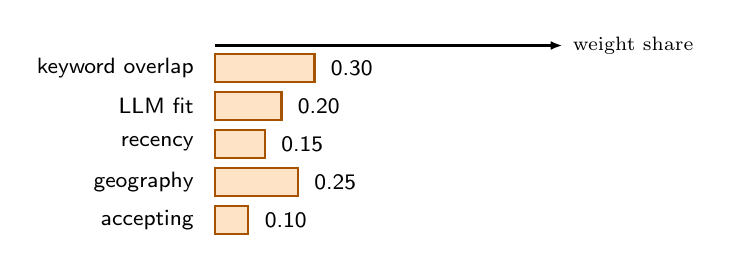
\begin{tikzpicture}[font=\footnotesize\sffamily, x=0.42cm, y=0.42cm]
  \foreach \lab/\w [count=\i from 0] in {keyword overlap/0.30, LLM fit/0.20, recency/0.15, geography/0.25, accepting/0.10} {
    \pgfmathsetmacro{\yi}{-(\i)*1.15}
    \pgfmathsetmacro{\bar}{\w*10}
    \draw[fill=orange!22, draw=orange!65!black, thick] (0,\yi) rectangle (\bar,\yi+0.85);
    \node[anchor=east, left=0.15cm] at (0,\yi+0.42) {\lab};
    \node[anchor=west] at (\bar+0.2,\yi+0.42) {\w};
  }
  \draw[thick, -{Latex[length=1.5mm]}] (0,1.1) -- (10.5,1.1) node[right, font=\scriptsize] {weight share};
\end{tikzpicture}
\caption{Composite relevance score $s=\sum_i w_i s_i$: bar length is $w_i$ (Section~4, step~9).}
\label{fig:score-weights}
\end{figure}

\begin{figure}[htbp]
\centering
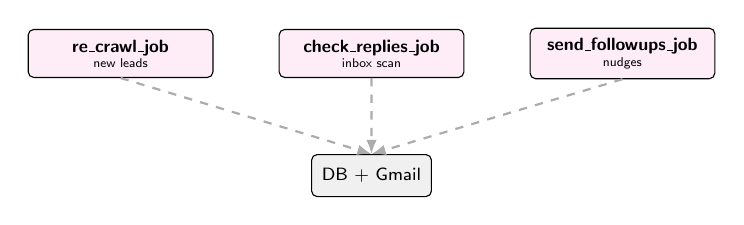
\begin{tikzpicture}[
  scale=0.92, transform shape,
  font=\scriptsize\sffamily,
  job/.style={diagnode, fill=magenta!7, minimum width=2.55cm, minimum height=0.62cm, align=center},
  hub/.style={diagnode, fill=gray!12, minimum width=1.55cm, minimum height=0.58cm},
]
  \node[job] (j1) at (0,0) {\textbf{re\_crawl\_job}\\[-2pt]{\tiny new leads}};
  \node[job, right=0.9cm of j1] (j2) {\textbf{check\_replies\_job}\\[-2pt]{\tiny inbox scan}};
  \node[job, right=0.9cm of j2] (j3) {\textbf{send\_followups\_job}\\[-2pt]{\tiny nudges}};
  \node[hub, below=1.05cm of j2] (hub) {DB + Gmail};
  \foreach \j in {j1,j2,j3}
    \draw[diagarr, dashed] (\j.south) -- (hub.north);
\end{tikzpicture}
\caption{Autonomous scheduler jobs (APScheduler) and their shared sinks after the user enables automation (Section~4, step~14).}
\label{fig:scheduler-jobs}
\end{figure}

% ---------------------------------------------------------------------------
\section{Control flow and routing logic}

\subsection{LangGraph conditional edges}
Figure~\ref{fig:langgraph} sketches the graph; the bullets spell out the routing predicates.

\begin{figure}[htbp]
\centering
\resizebox{\linewidth}{!}{%
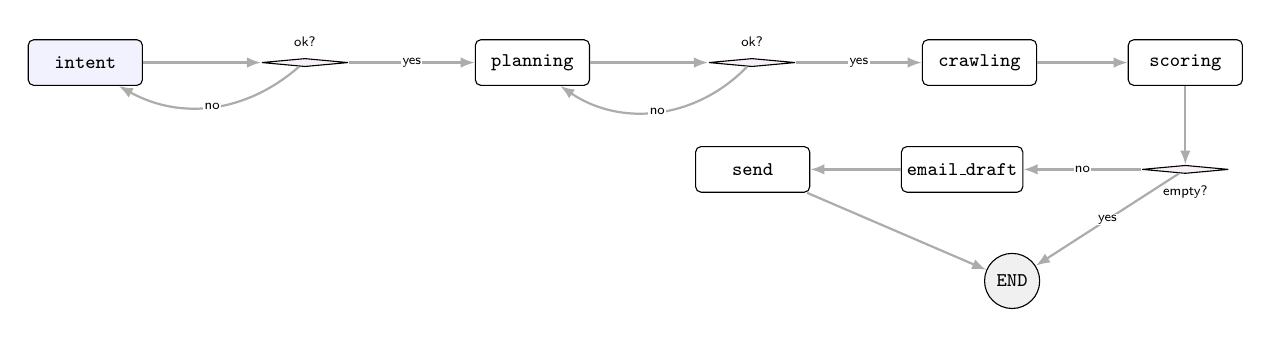
\begin{tikzpicture}[
  font=\scriptsize\ttfamily,
  nd/.style={diagnode, minimum width=1.45cm, minimum height=0.58cm, inner sep=2pt},
  diam/.style={draw, diamond, aspect=2, inner sep=1pt, minimum width=1.1cm, fill=violet!6},
  every edge quotes/.style={fill=white, inner sep=0.5pt, font=\tiny\sffamily},
]
  \node[nd, fill=blue!5] (I) {intent};
  \node[diam, right=1.5cm of I] (Ic) {};
  \node[above=0.02cm of Ic] {\sffamily\tiny ok?};
  \node[nd, right=1.6cm of Ic] (P) {planning};
  \node[diam, right=1.5cm of P] (Pc) {};
  \node[above=0.02cm of Pc] {\sffamily\tiny ok?};
  \node[nd, right=1.6cm of Pc] (C) {crawling};
  \node[nd, right=1.15cm of C] (S) {scoring};
  \node[diam, below=1.0cm of S] (Sz) {};
  \node[below=0.02cm of Sz] {\sffamily\tiny empty?};
  \node[nd, left=1.5cm of Sz] (E) {email\_draft};
  \node[nd, left=1.15cm of E] (Sn) {send};
  \node[nd, circle, below=1.0cm of Sz, xshift=-2.2cm, inner sep=1pt, minimum size=0.7cm, fill=gray!12] (END) {END};

  \draw[diagarr] (I) -- (Ic);
  \draw[diagarr] (Ic) to["yes"] (P);
  \draw[diagarr] (Ic) to[bend left=35, "no"] (I);
  \draw[diagarr] (P) -- (Pc);
  \draw[diagarr] (Pc) to["yes"] (C);
  \draw[diagarr] (Pc) to[bend left=40, "no"] (P);
  \draw[diagarr] (C) -- (S);
  \draw[diagarr] (S) -- (Sz);
  \draw[diagarr] (Sz) to["yes"] (END);
  \draw[diagarr] (Sz) to["no"] (E);
  \draw[diagarr] (E) -- (Sn);
  \draw[diagarr] (Sn) -- (END);
\end{tikzpicture}%
}
\caption{LangGraph-style routing (Section~5). Diamonds abbreviate \texttt{intent.confirmed}, \texttt{plan.confirmed}, and \texttt{shortlisted} empty; \texttt{send} may be emulated in CLI runs.}
\label{fig:langgraph}
\end{figure}

\begin{itemize}[noitemsep]
  \item After \texttt{intent}: if \texttt{intent.confirmed}, go to \texttt{planning}; else loop \texttt{intent}.
  \item After \texttt{planning}: if \texttt{plan.confirmed}, go to \texttt{crawling}; else loop \texttt{planning}.
  \item After \texttt{crawling}: unconditional edge to \texttt{scoring}.
  \item After \texttt{scoring}: if \texttt{shortlisted} is empty, \texttt{END}; else \texttt{email\_draft}.
  \item After \texttt{email\_draft}: edge to \texttt{send} (CLI graph uses \texttt{send\_emulated} for simulation), then \texttt{END}.
\end{itemize}

\subsection{Supervised CLI loop (\texttt{run\_supervised\_loop})}
Streams graph events and pauses for terminal input when intent or plan is not yet confirmed, injecting the next \texttt{human\_input} and resuming---a lightweight human-in-the-loop pattern without full LangGraph interrupt nodes. Figure~\ref{fig:hil-loop} contrasts the two confirmation gates.

\begin{figure}[htbp]
\centering
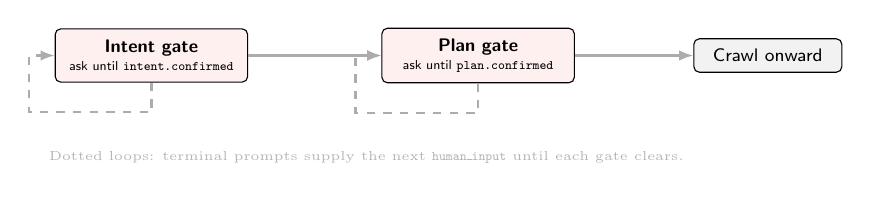
\begin{tikzpicture}[
  scale=0.94, transform shape,
  font=\scriptsize\sffamily,
  gate/.style={diagnode, fill=red!6, minimum width=2.6cm, minimum height=0.72cm, align=center},
]
  \node[gate] (g1) at (0,0) {\textbf{Intent gate}\\[-1pt]{\tiny ask until \texttt{intent.confirmed}}};
  \node[gate, right=1.8cm of g1] (g2) {\textbf{Plan gate}\\[-1pt]{\tiny ask until \texttt{plan.confirmed}}};
  \node[diagnode, fill=gray!10, right=1.6cm of g2, minimum width=2.0cm] (g3) {Crawl onward};

  \draw[diagarr] (g1) -- (g2);
  \draw[diagarr] (g2) -- (g3);

  \draw[diagarr, dashed] (g1.south) -- ++(0,-0.4) -| ($(g1.west)+(-0.35,0)$) |- (g1.west);
  \draw[diagarr, dashed] (g2.south) -- ++(0,-0.4) -| ($(g2.west)+(-0.35,0)$) |- (g2.west);

  \node[font=\tiny, text=gray!58, below=0.8cm of g1.south west, anchor=north west, xshift=-0.2cm]
    {Dotted loops: terminal prompts supply the next \texttt{human\_input} until each gate clears.};
\end{tikzpicture}
\caption{Human-in-the-loop pattern in the supervised CLI before expensive crawling.}
\label{fig:hil-loop}
\end{figure}


% ---------------------------------------------------------------------------
\section{Key design decisions}

\begin{description}[style=nextline,font=\normalfont\bfseries]
  \item[Slot-filling vs.\ free chat] Clarification is template-driven and JSON-parseable, reducing ambiguity before expensive crawl/send steps.
  \item[Hybrid relevance] Lexical overlap plus an LLM fit score balances interpretability with semantic matching when CV signals exist.
  \item[Email quality gates] Salutation guards, keyword sanitization, word-count targets, and a critique pass mitigate malformed or generic outreach.
  \item[Persistence boundaries] Session intent/plan in JSON; drafts and sent mail in SQLite; OAuth tokens external to this report.
\end{description}

% ---------------------------------------------------------------------------
\section{Documented live run (exact session log)}



\IfFileExists{transcript_ascii.txt}{%
\begin{tcbinputlisting}{
  enhanced,
  breakable,
  listing only,
  listing file={transcript_ascii.txt},
  title={\textbf{Complete session log} --- exact transcript},
  fonttitle=\bfseries\small,
  coltitle=black,
  colbacktitle=gray!12,
  attach boxed title to top left={yshift=-1mm, xshift=3mm},
  boxed title style={empty, size=minimal, top=1mm, bottom=1mm},
  colback=gray!6,
  colframe=black!55,
  boxrule=0.9pt,
  arc=2pt,
  outer arc=2pt,
  left=5pt,
  right=5pt,
  top=4pt,
  bottom=4pt,
  before skip=0.75em,
  after skip=1.25em,
  listing options={
    style=runlog,
    breaklines=true,
    columns=fullflexible,
  },
}
\end{tcbinputlisting}%
}{%
  \begin{center}
  \fbox{\begin{minipage}{0.92\linewidth}
  \textbf{Missing file \texttt{transcript\_ascii.txt}.} On Overleaf, upload \texttt{transcript\_ascii.txt} into the \emph{same project folder} as this \texttt{.tex} file. Copy it from the repository root.
  \end{minipage}}
  \end{center}%
}

% ---------------------------------------------------------------------------
\section{Limitations and operational notes}

\begin{itemize}[noitemsep]
  \item Web scraping depends on page structure and rate limits; some faculty pages yield incomplete profiles.
  \item Search API keys and LLM backends must be configured via environment variables (\texttt{config.py}); the stack may use Groq or other providers as wired in code.
  \item Autonomous mode sends real email; users should verify legal, institutional, and etiquette constraints before enabling schedulers.
\end{itemize}

% ---------------------------------------------------------------------------
\section{Conclusion}

The project implements a coherent pipeline from natural-language goals to structured state, approved plans, grounded discovery, ranked candidates, and supervised email generation, with a path toward scheduled re-crawling, reply tracking, and follow-ups. The 14-step workflow above matches the intended product narrative and aligns with the main classes and modules in the repository. Figures throughout Sections~2--6 visualize architecture, repository layout, CLI phases, data paths, intent slot-filling, email lifecycle, crawl/score pipelines, scheduler jobs, LangGraph routing, and human-in-the-loop gates. Section~7 embeds the full supervised-session log verbatim (Game Theory / Punjab, India run) in a framed, page-breaking listing.

\end{document}
